\solution 
See Fig. \ref{fig:10/7/4/8Fig3}. From 
  \eqref{eq:10/7/4/8det2f}, $PQRS$ is a parallelogram.
\begin{align}
  %\label{eq:10/7/4/8det2f}
  \vec{P}  = 
 \myvec{3 \\2},\, 
 \vec{Q}  = \myvec{
 2 \\
 4 \\
 } ,\,
 \vec{R}  = \myvec{
 5 \\
 \frac{3}{2}
 }   
  ,\,
 \vec{S}  = \myvec{
 2\\
 -1 \\
 }   
 \\
	\implies 
 \brak{\vec{Q}-\vec{P}}^\top\brak{\vec{R}-\vec{Q}}  \neq 0
 \\
 \brak{\vec{R}-\vec{P}}^\top\brak{\vec{S}-\vec{Q}}  = 0
\end{align}
Therefore $PQRS$ is a rhombus.
\begin{figure}[H]
	\begin{center}
		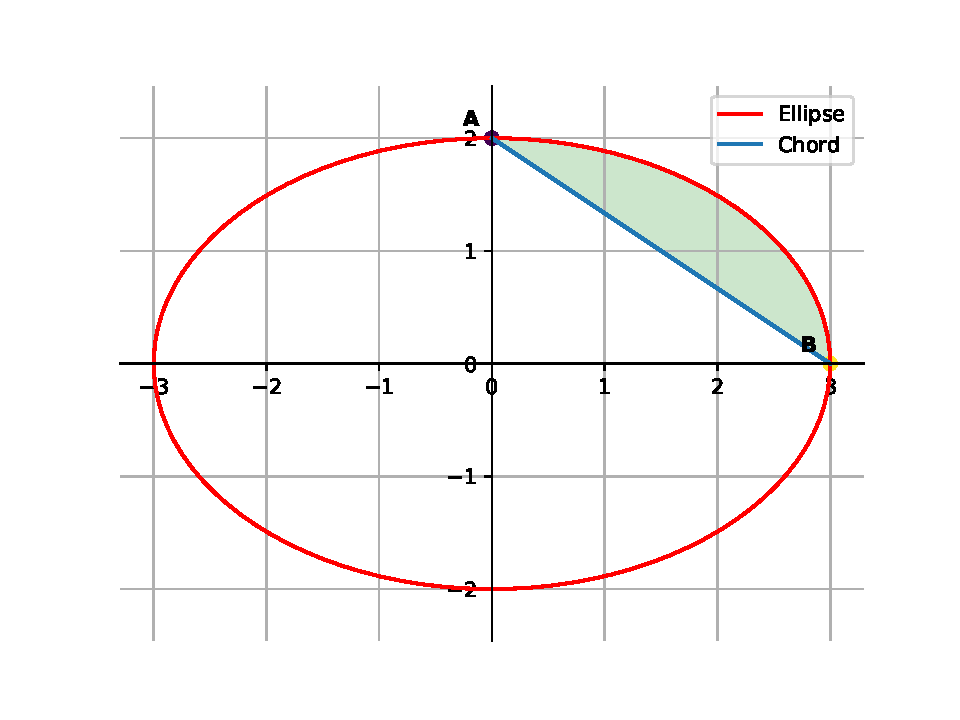
\includegraphics[width=0.75\columnwidth]{chapters/10/7/4/8/figs/fig.pdf}
	\end{center}
\caption{}
\label{fig:10/7/4/8Fig3}
\end{figure}

